% ---------------------------------------------------------------
% Ablation subsection: expert routing (EXPERIMENTS.md E6). Drafted
% 2026-09-22 from the repo's own numbers, NOT from memory:
%   arms, parity, within-pool balance   EXPERIMENTS.md E6; VARIANTS.md
%                                       A.2.moe_hardroute / A.2.moe_permod
%   stamp probes (0.589 -> 0.408, 69%,   MOE_ROUTING_REPORT.md, jobs
%     swap 0/11)                        178945 / 178946
%   bias arm (deltas 0.02-0.06, 0/12)   MOE_ROUTING_REPORT.md, jobs
%                                       179683 / 179684
%   purity, content probe               figures/plot_expert_purity.py,
%     (jobs 182681 shared / 182680 ours) figures/plot_content_probe.py
%   utilisation, deadliness             figures/plot_expert_load*.py,
%     (jobs 182681/182680 teacher-forced, figures/utilization_stats.py,
%      182747/182746 free-running)       figures/plot_load_distribution.py
%
% TERMINOLOGY is method.tex's: stream, frame, position, token,
% content/query token. The figure scripts said "per-modality gates";
% relabelled 2026-09-22 to "stream-specific routers" (the paper's word;
% "modality" is reserved for the general framework). "Shared router" is
% the ablation arm, never the design. The arm codes (A2, D1-D3) and
% run-dir markers (K4mg, hr, densecm) stay out of the prose.
%
% Preamble: \usepackage{amsmath} ONLY. No \paragraph headings. No
% amssymb, so no \mathbb; set memberships are prose.
%
% PLACEHOLDERS marked [X] are NOT yet settled and must not be guessed:
%   - every generation-quality number (the four-arm E1 chain,
%     eval_a2_moe_ablation.sbatch) -- the hard-partitioned and dense
%     arms are implemented and audited but NOT TRAINED as of this draft
%     (VARIANTS.md A.2.moe_hardroute: "training run not yet launched");
%   - the per-arm training budget: the shared checkpoint is the
%     50k-step cp4tar run, ours the 100k-step long run -- NOT budget-
%     matched; a matched shared run is an open decision (EXPERIMENTS.md
%     E6, "Budget-parity note");
%   - the stamp-share numbers were measured on the v1.2 checkpoint of
%     the OLD corpus (method_per_part_moe.tex header: "must be
%     re-measured on v5, where chord carries program 48"). They are the
%     only measurement there is and are printed, but re-run
%     analyze_moe_routing.sbatch with --probe identical / swap on the v5
%     shared checkpoint before submission and replace them.
%
% FIGURES (vector PDFs in midi_yinyang/figures/, rebuilt 2026-09-22):
%   fig:routing   expert_purity.pdf  +  content_probe.pdf   (two panels)
%   fig:load      load_distribution.pdf
%   supplementary / if space: expert_load.pdf, expert_load_freerun.pdf
%     (the per-cell heatmaps behind fig:load; every value annotated)
% ---------------------------------------------------------------
\subsection{Expert-routing ablation}
\label{sec:abl_routing}

Sec.~\ref{sec:permod_moe} routes every position with the router of its
own stream and defers two questions to this section: what a single
shared router keys on, and what the stream-specific routers do with the
capacity this frees. We compare four feed-forward designs that differ
only in how positions reach experts. \emph{Shared}: one $E \times d$
router scores every position. \emph{Stream-specific} (\sys):
$\mathbf{G}^{(x)}$ and $\mathbf{G}^{(y)}$ over one pool,
Eq.~\eqref{eq:permod_router}. \emph{Hard-partitioned}: stream $x$ may
reach only the first two experts and stream $y$ only the last two, the
other pair's logits masked before the softmax, as in modality-specific
expert designs~\cite{moma}; the balance term is computed within each
pair, so the arm is not penalised for a load it cannot produce.
\emph{Dense}: a single feed-forward layer of inner width $8d$, matching
the activated compute of two $4d$ experts. The three routed arms have
identical parameters and activated compute and share one warm start:
the two stream-specific routers are initialised as the same matrix, so
at step~0 the model \emph{is} the shared-router model, and the routers
diverge only as their streams' gradients differ. [X: per-arm training
budget.] Routing statistics below are read on a fixed held-out batch of
two songs, 384 frames each, giving about 770 positions per stream per
layer; a second independent batch reproduces every pattern reported.

We first ask what a shared router separates. Its expert preferences
differ strongly between the streams, with a mean $\ell_1$ distance of
$0.59$ between the mean routing distributions of stream-$x$ and
stream-$y$ positions (maximum $2$), which reads as modality
specialisation. Two probes attribute it. Duplicating the melody token
into the chord positions, so that the two streams carry identical
content and only their stream identity differs, retains $0.41$ of the
$0.59$: about $69\%$ of the separation is the mark that the per-stream
projections $\mathbf{W}^V_s$, $\mathbf{W}^O_s$ leave on every hidden
state, not the music. Exchanging the two streams' contents moves the
expert preferences with the content in none of the eleven usable
layers. A shared router thus spends its capacity relaying a distinction
the architecture has already made explicit. Offering it that
distinction for free, as a per-stream bias on its logits, changes
nothing: the trained bias differs between the streams by at most
$0.06$ logits and the router keeps reading the projections' mark. The
separation has to be removed from the router's job, not offered to it,
which is what Eq.~\eqref{eq:permod_router} does: within one stream
the mark is a constant input, and a constant cannot rank two
positions of that stream differently.

% fig:routing -- (a) expert_purity.pdf, (b) content_probe.pdf
\begin{figure}[t]
  \centering
  \begin{minipage}[t]{0.56\columnwidth}
    \centering
    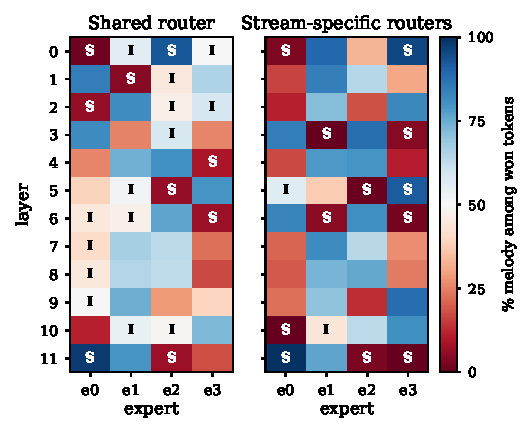
\includegraphics[width=\linewidth]{figures/expert_purity.pdf}
    \\ {\small (a)}
  \end{minipage}\hfill
  \begin{minipage}[t]{0.42\columnwidth}
    \centering
    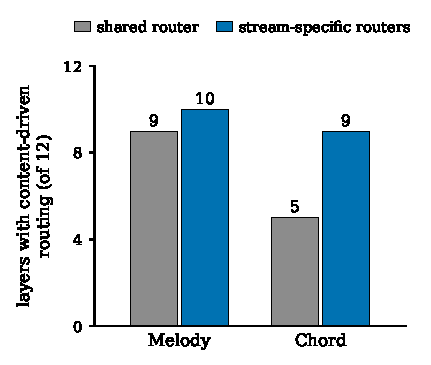
\includegraphics[width=\linewidth]{figures/content_probe.pdf}
    \\ {\small (b)}
  \end{minipage}
  \caption{Shared router versus stream-specific routers, same held-out
    batch. (a)~Expert purity: the share of melody among the positions
    each expert wins per layer. Poles are per-stream specialists (S,
    at most $10\%$ or at least $90\%$); the midpoint marks experts
    serving both streams (I, $40$--$60\%$). (b)~Layers, out of twelve,
    in which routing inside a stream follows the frame's register
    beyond a permutation null.}
  \label{fig:routing}
\end{figure}

Fig.~\ref{fig:routing}(a) shows where the freed capacity goes. We
measure the purity of an expert as the share of melody among the
positions it wins in a layer. Under the shared router the partition is
soft: nine of the 48 expert--layer cells are specialists at $90\%$ or
beyond, and fourteen sit within $10$ points of the base rate. Under
stream-specific routers the same pool becomes markedly more
stream-selective, twelve specialist cells and two mixed ones, with the
mean distance from the base rate rising from $22$ to $32$ points, and
the split is learned rather than imposed: no expert was assigned to a
stream, three layers pair a melody specialist with a chord specialist,
and the remaining experts serve both streams. Fig.~\ref{fig:routing}(b)
asks whether routing then follows the music. Inside each stream we
split the frames into terciles of register and compare the terciles'
mean routing distributions against a shuffle null (95th percentile of
twenty permutations). For melody, both routers are near the ceiling,
nine and ten layers of twelve; the shared router's content channel
already served melody. For chord, the shared router clears the null in
five layers and the stream-specific routers in nine: with one weight
matrix, chord content competed with the stream mark and with melody
structure for the same rows, and lost.

% fig:load -- load_distribution.pdf
\begin{figure}[t]
  \centering
  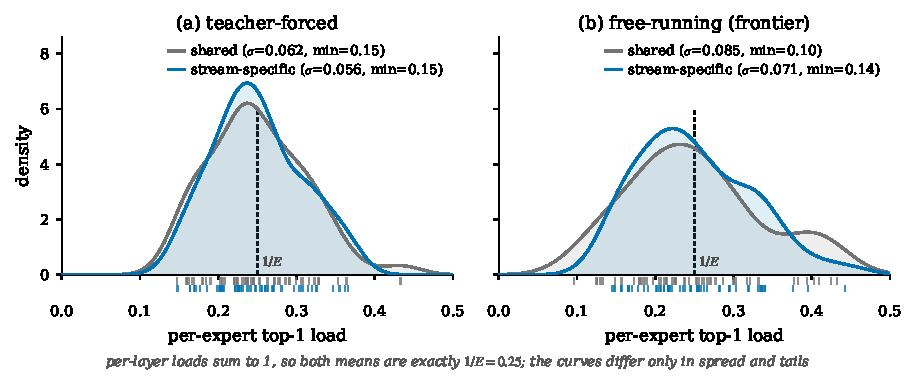
\includegraphics[width=\columnwidth]{figures/load_distribution.pdf}
  \caption{Distribution of the 48 per-expert top-1 loads (12 layers
    $\times$ 4 experts) per router design, (a)~teacher-forced on the
    held-out batch and (b)~free-running, over the routing decisions of
    the newest positions during generation. Per-layer loads sum to one,
    so both means are $1/E$ and only the spread differs.}
  \label{fig:load}
\end{figure}

Separate routers could starve an expert that one stream stops using.
They do not (Fig.~\ref{fig:load}). No expert is dead in either design,
teacher-forced or free-running, and we summarise the graded version as
deadliness, one minus the mean over layers of the smallest expert load
relative to $1/E$: $0.25$ for both designs under teacher forcing, and
$0.31$ against the shared router's $0.36$ when the model runs on its
own output, where the shared router's loads also spread wider
($\sigma = 0.085$ against $0.071$, minimum $0.10$ against $0.14$). The
stream-specific routers stay closer to balanced exactly where a
generator lives.

% Generation-quality table: four arms on the E1 primary endpoints,
% same prompts and decode settings, BASELINE = the shared arm
% (eval_a2_moe_ablation.sbatch). Every entry is [X] until the
% hard-partitioned and dense arms have trained and the chain has run.
\begin{table}[t]
  \caption{Generation quality of the four routing designs on the
    primary endpoints of Sec.~\ref{sec:evaluation}, same prompts and
    decode settings [X: songs, samples]. Mean$\pm$s.e.m.\ over songs.}
  \label{tab:routing_quality}
  \begin{center}
  \footnotesize
  \setlength{\tabcolsep}{4pt}
  \begin{tabular}{|l|c|c|c|c|}
  \hline
  \textbf{Metric} & \textbf{Dense} & \textbf{Shared} &
    \textbf{Hard-part.} & \textbf{Stream-spec.\ (ours)} \\
  \hline
  Harmonic rhythm JSD$^*$ ($\downarrow$) & [X] & [X] & [X] & [X] \\
  Chord-tone coverage$^*$ (ref.\ [X]) & [X] & [X] & [X] & [X] \\
  Survival, min over streams$^*$ ($\uparrow$) & [X] & [X] & [X] & [X] \\
  \hline
  \end{tabular}
  \end{center}
\end{table}

Table~\ref{tab:routing_quality} reports generation quality for the
four arms under the protocol of Sec.~\ref{sec:systems}. [X: The
hard-partitioned arm is the load-bearing contrast: it gives each
stream its own routing decision, as ours does, but forbids an expert
from serving both streams. If ours is better, the experts that serve
both streams do work a disjoint pool cannot express; if the two tie,
cross-stream expert sharing is not load-bearing on this corpus and the
mechanism result above stands on its own. The dense arm tells whether
routing is load-bearing at all; a deficit confined to the stream
grammar metrics would say that the experts carry the per-stream
grammars.]
